%template for simulation report

\newpage

\section{G54.1+0.3 pulsar wind nebula}

\textbf{Object Description:} G54.1+0.3 pulsar and nebula

\textbf{Simulation Period:} April 2011

\textbf{NuSIM revision:} 260

\textbf{Science Team contact:} Stephen Reynolds

\textbf{NuSIM configuration file:} G54.1.multispectrum.cfg

\textbf{Exposure time:} 200 ks

\textbf{Input Source:} 
The original Chandra image (G54.1.image.fits) was converted into the 3Ddat format (G45.1.3Ddat).
The inner 20 arcsec have a flux of $F = 7.9\cdot10^{-6}\,(E/10\,keV)^{-2.0}\,ph\,cm^{-2}\,s^{-1}\,keV^{-1}$, the rest a flux of $F = 4.1\cdot10^{-6}\,(E/10\,keV)^{-2.2}\,ph\,cm^{-2}\,s^{-1}\,keV^{-1}$.

\textbf{Tiling Method:} Single pointing

\textbf{OA Database Version:} 008

\textbf{Mast Bend Database:} SAA90

\textbf{Simulation notes:} While the input image has been cut down to the PWN as good as possible, this cut is circular and not perfect. The remainig (Chandra) background around the pulsar has the same flux as the pulsar and counts towards the total flux.

\textbf{Status:} 
Redo when improved depth cuts are available

\textbf{Location and name of simulation output:} resource/examples/G54.1+0.3

\begin{figure}[h]
\begin{center}
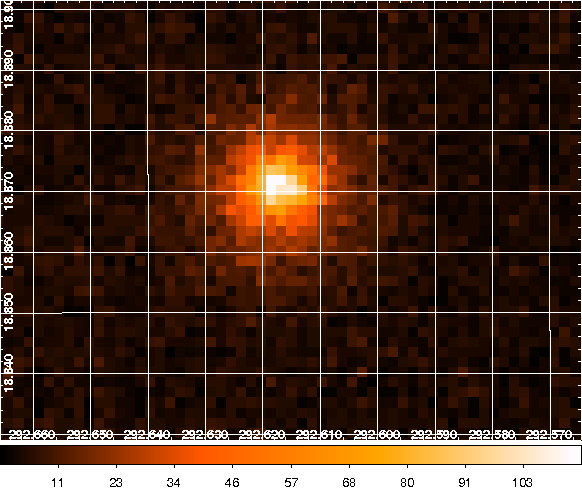
\includegraphics[width=12cm]{G54.1+0.3/G54.png}
\caption{G54.1+0.3 PWN between 10 and 40 keV after 200 ks observation time}
\label{Vela} 
\end{center}
\end{figure}

